%\documentclass[../Manuscrit.tex]{subfiles}
\documentclass[../eBook.tex]{subfiles}

\begin{document}
  \phantomsection
  \addchapterline{Situation}
  \subsection*{Situation}
    \paragraph{}Le village de \textit{\textbf{Sermaise}} est situé à 6 \textit{kilom.} 200 de Dourdan son chef-lieu de canton et à 51 \textit{kilom.} 103 de Paris.
    \paragraph{}Le territoire de la commune a fait partie de l'ancien Hurepoix \og \textit{Uripiorium felix regio} \fg{}, l'heureux pays de l'Hurepoix, disaient les anciens géographes en parlant de la province à laquelle ils donnaient Dourdan pour capitale ; et à leurs yeux cette contrée où s'entremêlaient bois, prairies, moissons, vignes et vergers était un contraste, un dédommagement à côté de la région moins favorisée du Gâtinais.
    \paragraph{}La commune occupe comme celle de Roinville dont elle semble le prolongement, le fond et les versants d'une vallée. De Roinville à Sermaise, et au-delà, la route est parfois bordée de frais ombrages suivant le cours de l'Orge, de bois marécageux, de prés humides. Sermaise, un peu caché quoique près de cette route de Dourdan à Saint-Chéron, est un village aux maisons peu nombreuses dont l'emplacement mal nivelé accuse un bouleversement du sol. En effet, Sermaise a failli être détruit plusieurs fois par les inondations dont les deux plus connues sont celles de 1780 et 1829.

  \phantomsection
  \addchapterline{Communes limitrophes}
  \subsection*{Communes limitrophes}
    \paragraph{}Le territoire de Sermaise et de ses nombreux hameaux \&  écarts est limité par les communes du Val-Saint-Germain au nord, de Saint-Chéron au nord-est et à l'est, de Villeconin au sud-est, de Boissy-le-Sec au sud, de Roinville à l'ouest.

  \phantomsection
  \addchapterline{Population}
  \subsection*{Population}
    \paragraph{}La population de la commune est actuellement de 514 habitants et se partage comme suit : Sermaise-chef-lieu, \textit{148 individus, 39 maisons} ; Blancheface, \textit{151 individus, 50 maisons} ; le Mesnil, \textit{76 individus, 28 maisons} ; Montflix, \textit{43 individus, 11 maisons} ; Mondétour, \textit{28 individus, 7 maisons} ; la Charpenterie, \textit{5 individus, 3 maisons} ; le Tertre, \textit{15 individus, 1 maison} ; Haute-Minière, \textit{7 individus, 1 maison} ; la Mercerie, \textit{5 individus, 1 maison} ; la Rachée, \textit{6 individus, 2 maisons} ; la Jeulerie, \textit{10 individus, 2 maisons} ; la Maison Blanche, \textit{11 individus, 2 maisons} ; Villeneuve, \textit{6 individus, 1 maison} ; Bellenger, \textit{3 individus, 1 maison}.
    \paragraph{}Le nombre des habitants de Sermaise était de 168 vers 1275, de 400 en 1676, de 596 en 1743, de 616 en 1806, de 666 en 1824, de 572 en 1846, de 560 en 1856, de 549 en 1866, de 471 en 1891.

  \phantomsection
  \addchapterline{Superficie}
  \subsection*{Superficie}
    \paragraph{}En 1820, lors de la confection du cadastre, le territoire de la commune se divisait comme suit :
    \begin{center}
      Terres labourables\dotfill 967 \textit{ha} 6785\\
      Vignes\dotfill 61 \textit{ha} 8330\\
      Bois\dotfill 190 \textit{ha} 3650\\
      Jardins\dotfill 8 \textit{ha} 51~~~~\\
      Prés\dotfill 45 \textit{ha} 0660\\
      Aulnaies\dotfill 8 \textit{ha} 4065\\
      Objets d'agrément\dotfill 2 \textit{ha} 3640\\
      Pâtures plantées ou non plantées\dotfill  1 \textit{ha} 9640\\
      Friches plantées\dotfill 2 \textit{ha} 3035\\
      Oseraies\footnote{\textit{NDLR} --- Terrains plantés d'osiers}\dotfill 0 \textit{ha} 9835\\
      Mares\dotfill 0 \textit{ha} 98~~~~\\
      Murgers, friches nues ou terres vaines\dotfill 27 \textit{ha} 6860\\
      Propriétés bâties\dotfill 8 \textit{ha} 3860\\
      Divers (chemins, cours d'eau)\dotfill 33 \textit{ha} 5625
    \end{center}
    \hfill Total\makebox[2cm]{\dotfill} 1360 \textit{ha} 0175
    \paragraph{}Dans le courant du siècle, l'aspect du sol a été quelque peu modifié ; on peut aujourd'hui répartir le territoire de la manière suivante :

    \phantomsection
    \addsectionline{Superficie exploitée}
    \subsubsection*{Superficie exploitée}
      \begin{center}
        Terres labourables\dotfill  990 \textit{ha} 6937\\
        Prairies naturelles, herbages \& pâturages\dotfill  45 \textit{ha} 0660\\
        Vignes\dotfill 3 \textit{ha} 0000\\
        Jardins de particuliers\dotfill 8 \textit{ha} 5100\\
        Jardins de plaisance, parcs\dotfill 2 \textit{ha} 3640\\
        Bois \& forêts\dotfill 218 \textit{ha} 6007\\
      \end{center}
      \hfill Total\makebox[2cm]{\dotfill} 1268 \textit{ha} 2344

    \phantomsection
    \addsectionline{Superficie non exploitée}
    \subsubsection*{Superficie non exploitée}
      \begin{flushleft}
        Landes, pâtres bruyères\dotfill 31 \textit{ha} 9535\\
        Terrains marécageux\dotfill 9 \textit{ha} 3900\\
        Voies de communications, cours d'eau et constructions\linebreak{} n'ayant pas le caractère rural\dotfill 50 \textit{ha} 5096\\
      \end{flushleft}
      \hfill Total\makebox[2cm]{\dotfill} 91 \textit{ha} 8531

  \phantomsection
  \addchapterline{Altitude}
  \subsection*{Altitude}
    \paragraph{}La place de Sermaise-village est à 84 \textit{m} 401 au dessus du niveau de la mer. Le passage à niveau de Haute-minière sur le chemin de fer de Paris à Tours par Vendôme est coté 91 \textit{m} 584.

  \phantomsection
  \addchapterline{Nature du sol et climat}
  \subsection*{Nature du sol et climat}
    \paragraph{}Le sol est sableux dans les pentes, argilo-sableux dans le fond de la vallée, de composition mixte (sable, marne \& argile) dans les prairies. On trouve quelques bancs d'argile, de calcaire grossier et de tuf\footnote{\textit{NDLR} --- Type de roche à structure vacuolaire, ici d'origine sédimentaire formé par la précipitation de carbonate de calcium à partir d'eau} dans le versant sud.
    \paragraph{}Les crêtes des versants présentent un peu de meulière recouverte d'une couche arable de faible épaisseur (plateau du Tertre, Butte du Mesnil). Nous respirons ici un air vif mais sain, en raison de la nature du sol et de son abondante végétation. Les gelées printanières se font surtout sentir dans la vallée.
    \begin{center}
      \begin{figure}[!ht]
        \ifthenelse{\equal{\colorspace}{CMYK}}{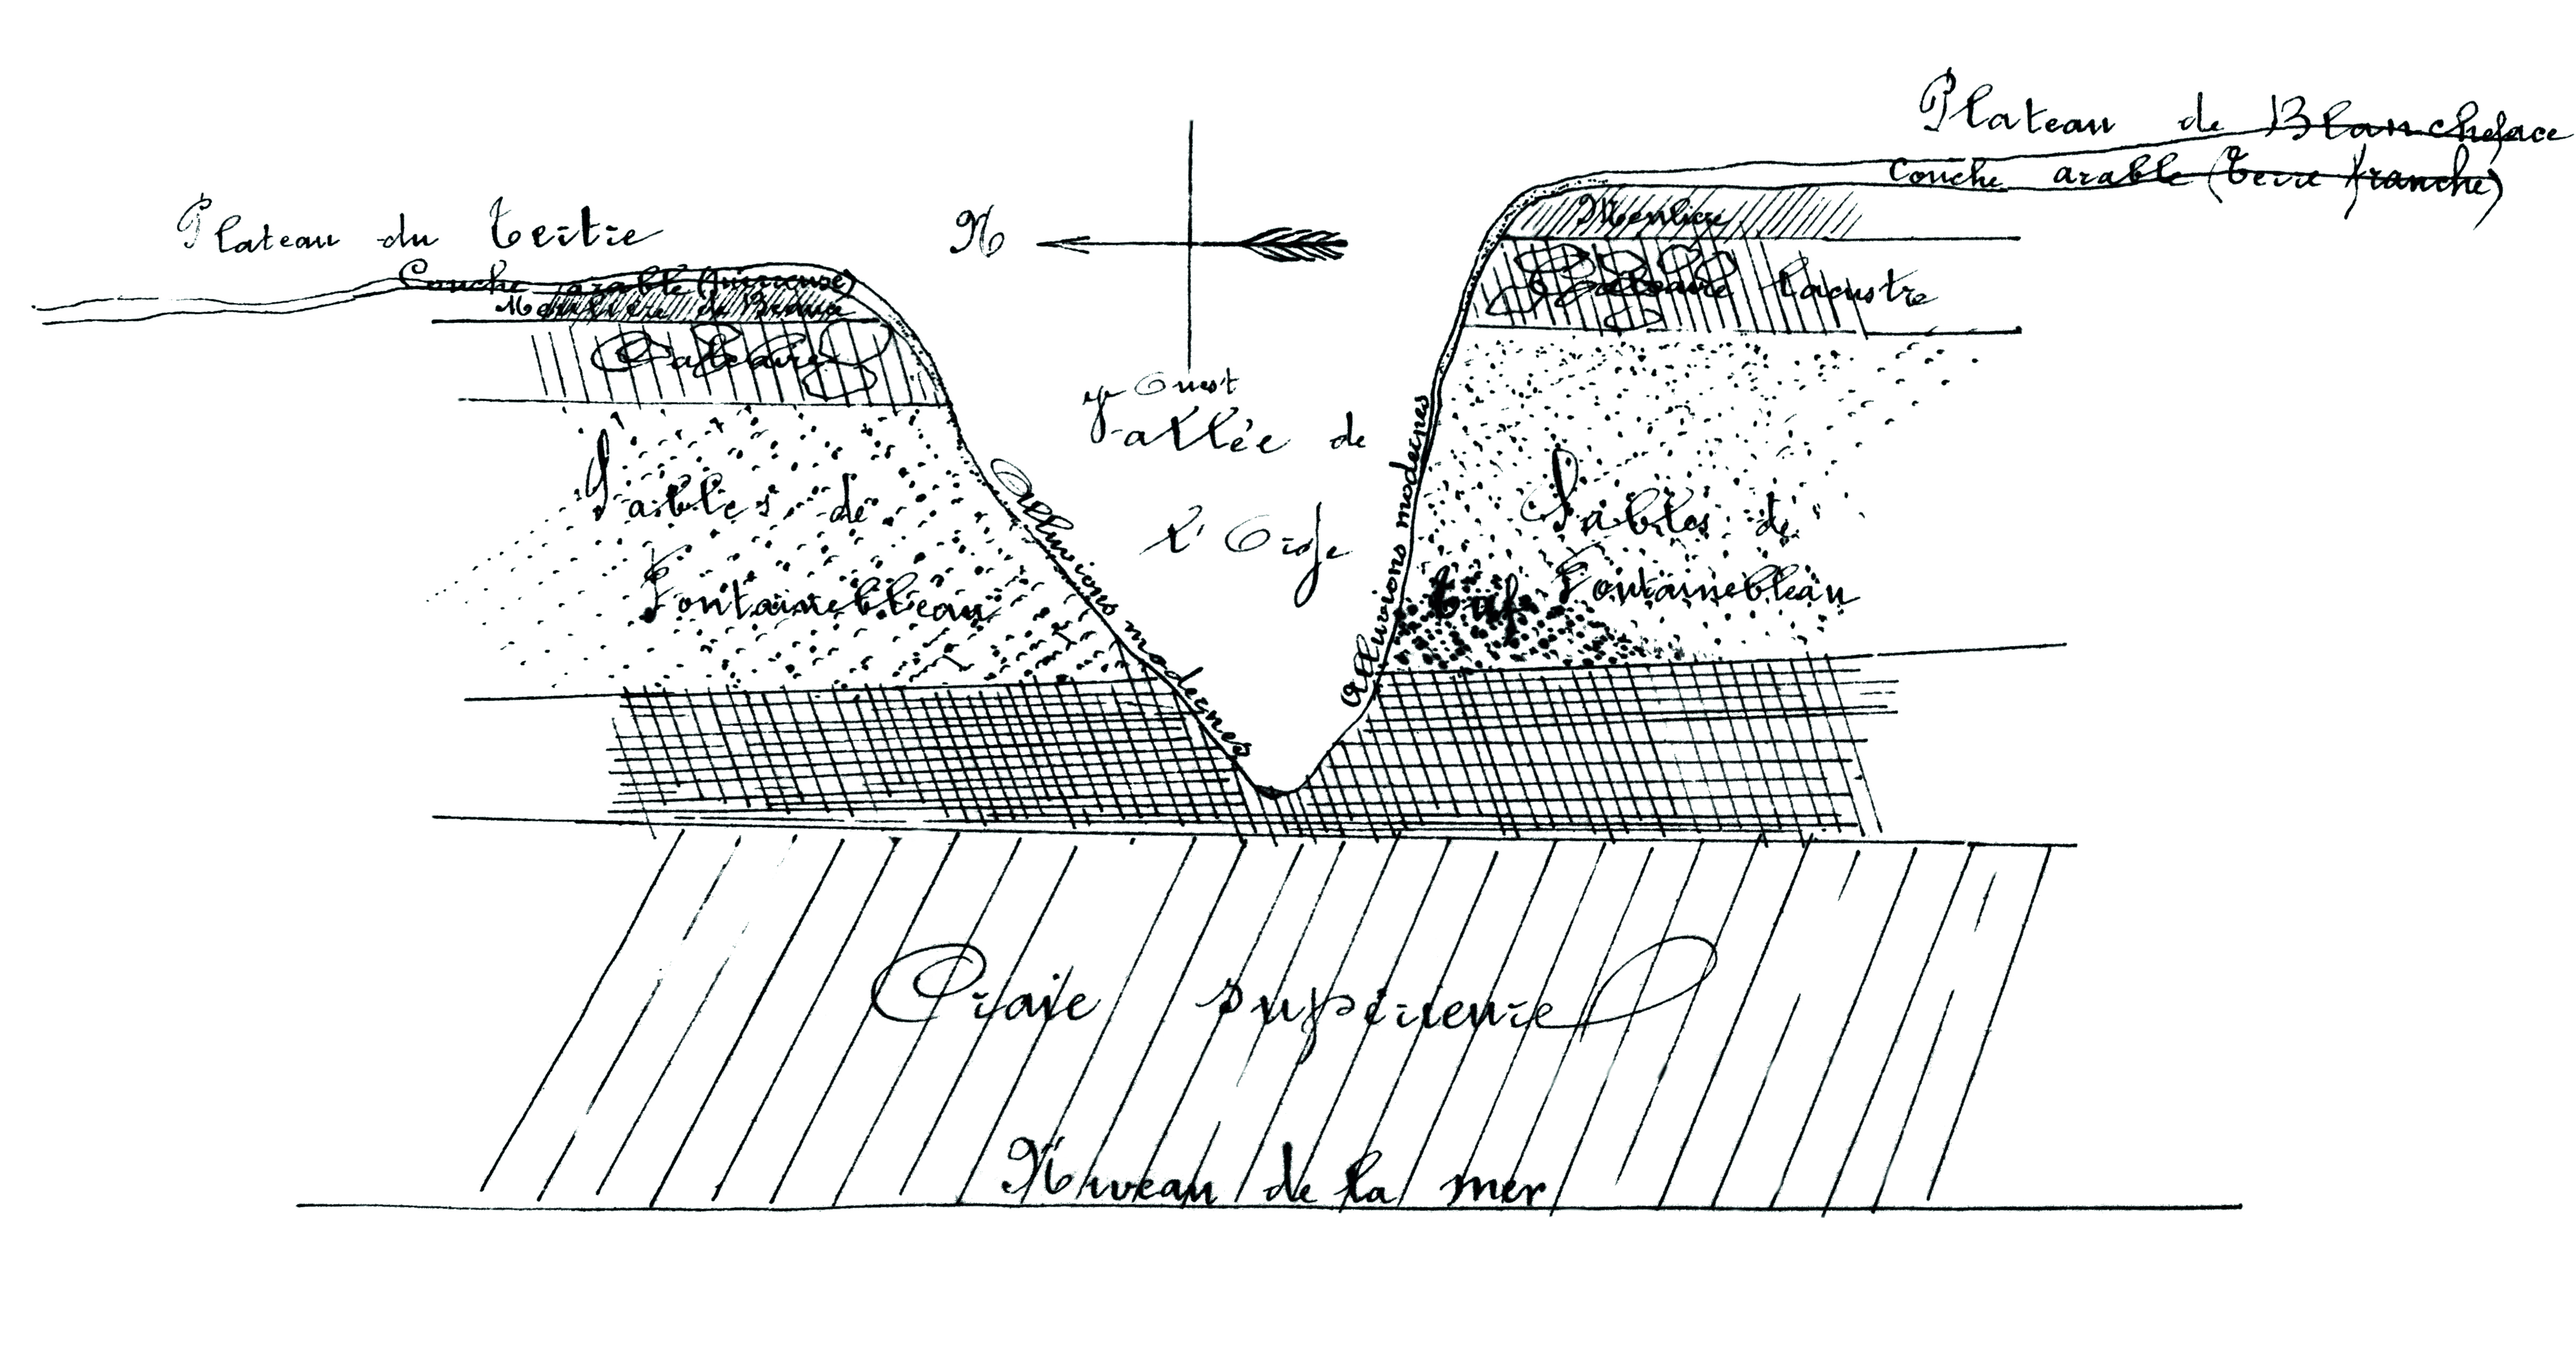
\includegraphics[width=\textwidth]{CMYK/02-geo-01-coupe.jpg}}{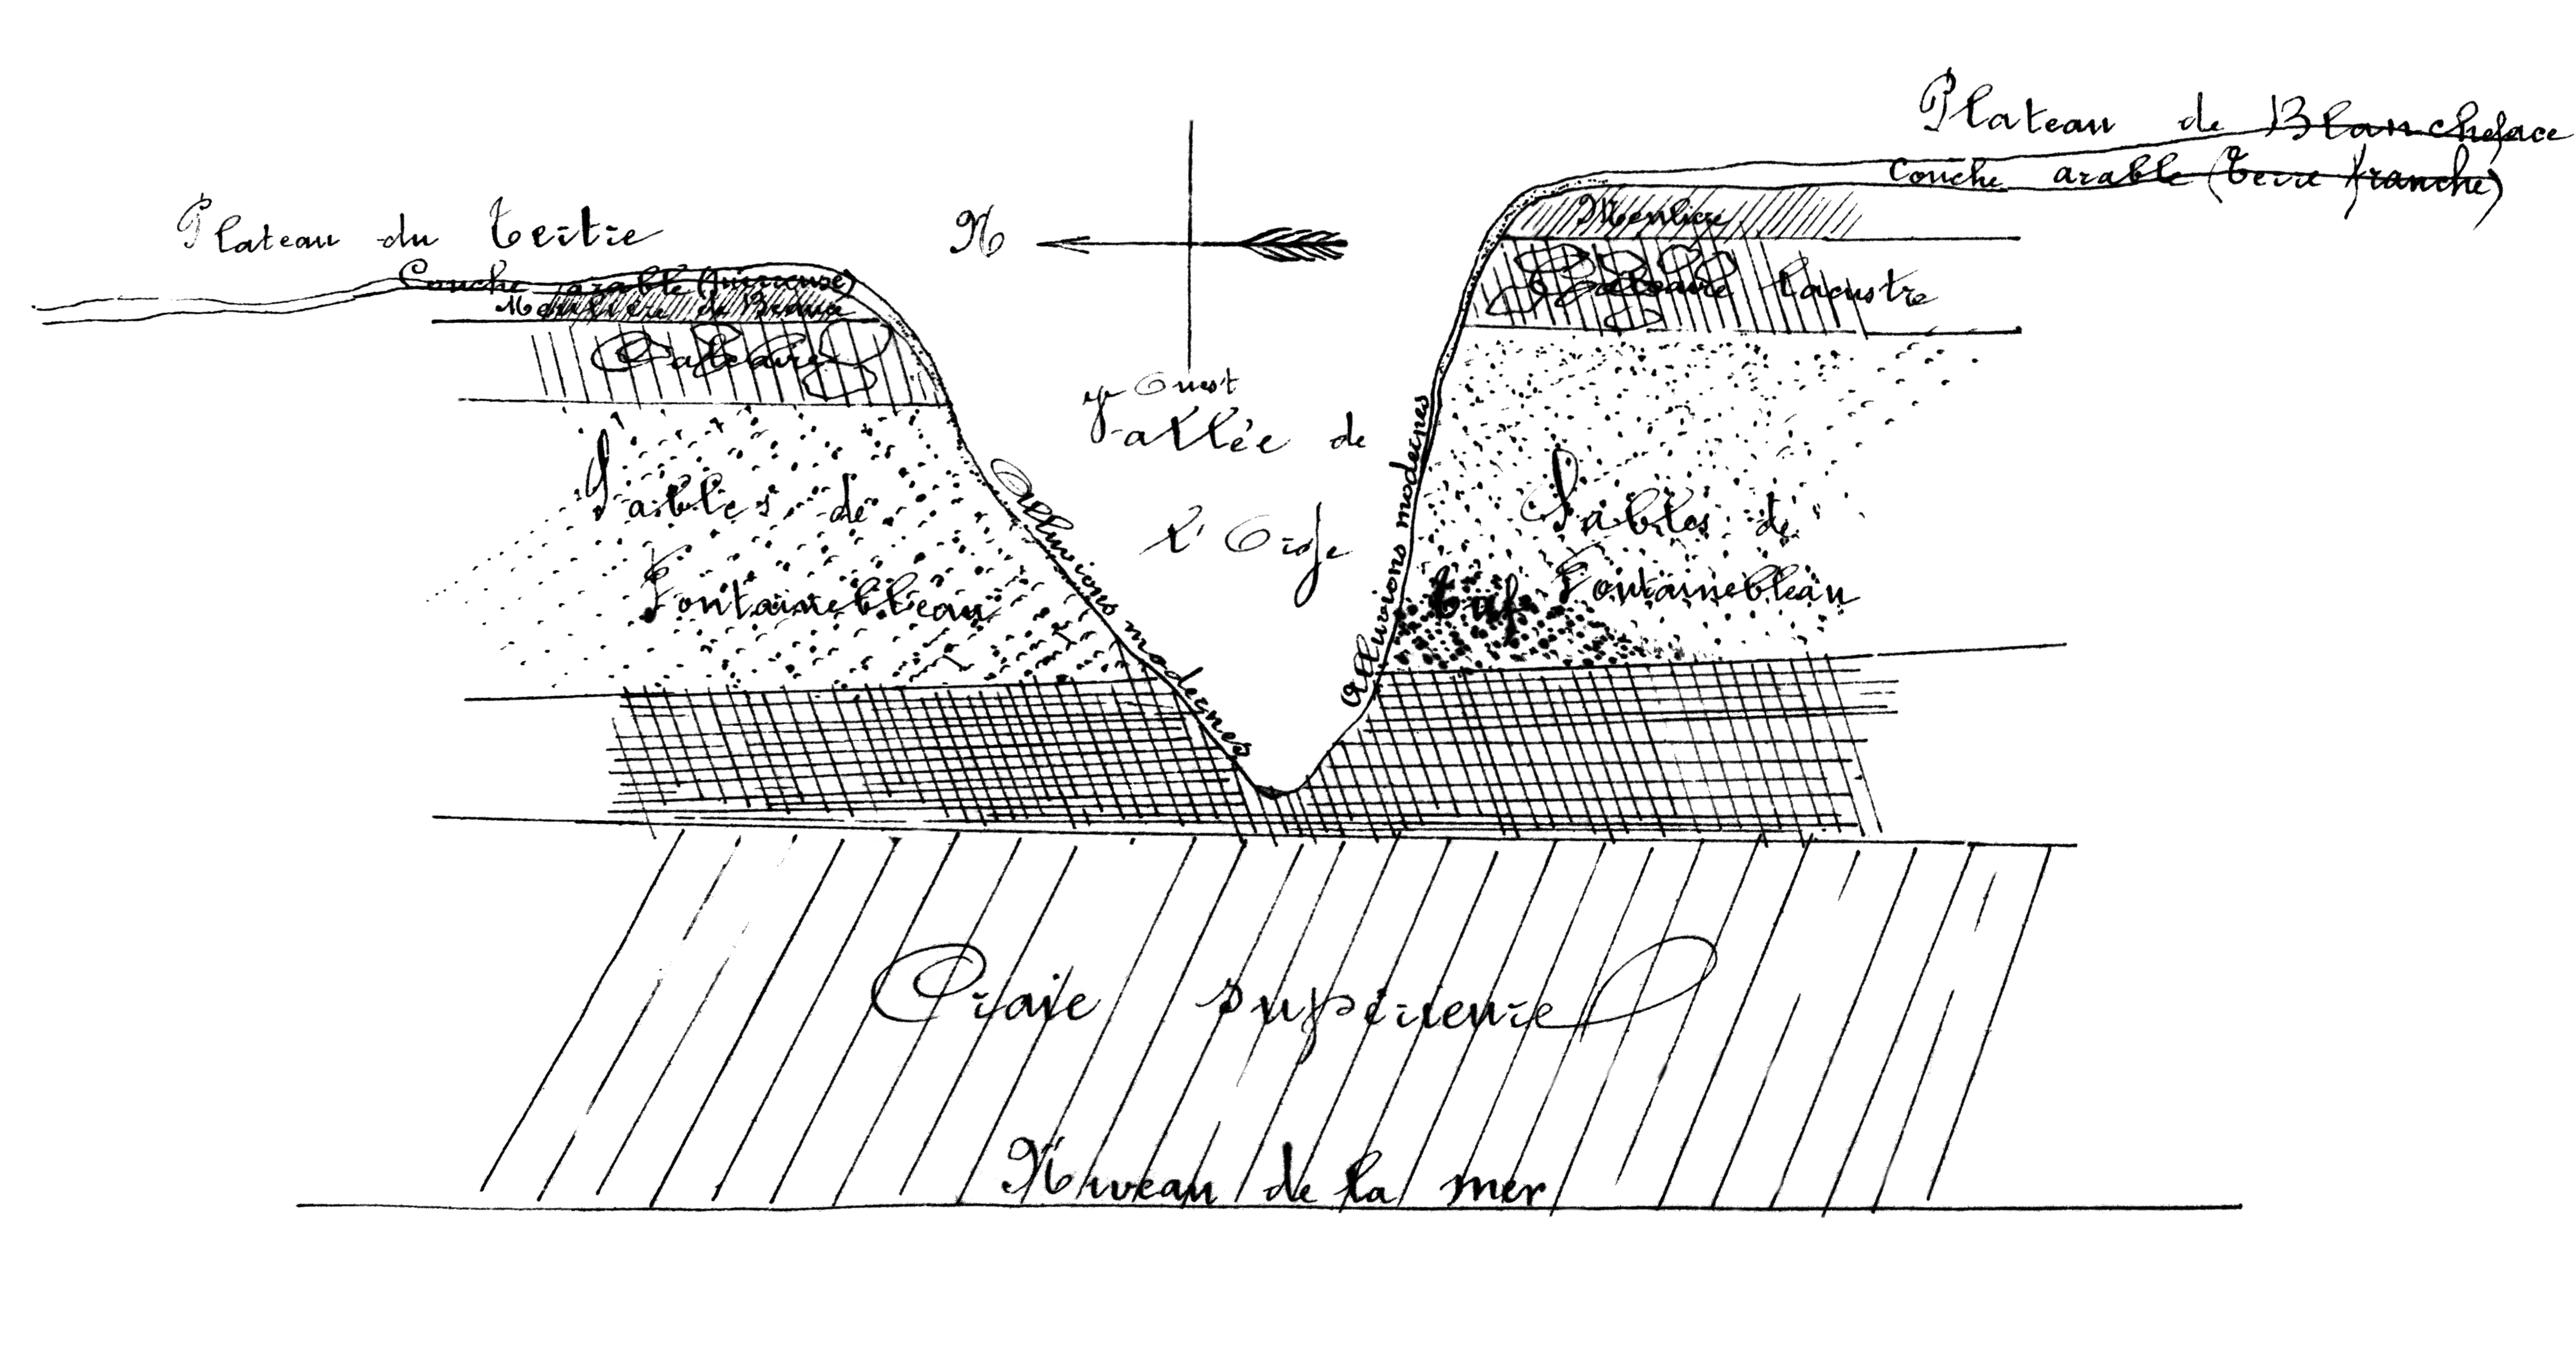
\includegraphics[width=\textwidth]{RGB/02-geo-01-coupe.png}}
        \caption*{Coupe géologique}
      \end{figure}
    \end{center}

  \phantomsection
  \addchapterline{Relief}
  \subsection*{Relief}
    \paragraph{}Le territoire de Sermaise est très accidenté. Sur le versant sud de la vallée de l'Orge on remarque les hauteurs de Villeneuve et de Mondétour, les hauteurs de Sermaise (Butte à la Blotte, bois de Graville), la butte du Bois du Croc, les buttes de Locandry ou du Mesnil. Au-delà des pentes du versant sud se trouvent les plaines fertiles de Mondétour, de Blancheface et du Mesnil. Montflix est à l'extrémité sud-est du territoire, à 4 \textit{kilom.} du chef-lieu.
    \paragraph{}Il appartient au versant ouest de la vallée de la Renarde, dite rivière de Souzy où descendent ses eaux par un ravin. Sur la rive gauche de l'Orge, en face du village de Sermaise se dresse la butte du Tertre. Il y a encore les pentes de la Bretonnière et de la Duboiserie. Derrière le Tertre on aperçoit la haute plaine ou plateau du même nom qui fait partie de la vaste propriété du Marais.

  \phantomsection
  \addchapterline{Hydrographie}
  \subsection*{Hydrographie}
    \paragraph{}Sermaise est traversé de l'ouest à l'est par la rivière d'Orge qui pénètre dans le territoire au lieu dit Moulin Rocher, passe à Bellenger, à Sermaise-village, à la Mercerie, près de la Charpenterie, à la Rachée, et rentre dans la commune de Saint-Chéron.
    \paragraph{}Quelques fossés, boëles \& morts-rûs ou bras-morts se détachent du cours principal de la rivière dont le lit naturel a été déplacé en maints endroits lors de l'installation des anciens moulins de Bellenger, de la Mercerie et de la Rachée (aujourd'hui usine).
    \paragraph{}Sur la rive droite de l'Orge arrivent quelques ravins : celui de Mondétour, ceux du Bois-Clair et du Bois du Cive, celui de Moque-Bouteille ou des buttes de Locandry, le ruisseau de la Rachée.
    \paragraph{}Sur la rive gauche on peut citer : le ruisseau de la Nation qui passe sous le chemin de fer et sous la route de Dourdan pour rejoindre l'Orge en aval de Bellenger ; le ravin de l'Etang qui descend des pentes de la Bretonnière. Les sources de la fontaine au Lait clair, de l'aulnaie des Petites fontaines et de la Fontaine du Croc (rive droite) ne sont pas assez abondantes pour former même un ruisseau ; leurs eaux se perdent dans les terres.
    \paragraph{}Le village de Sermaise est assez bien pourvu d'eau. Il n'en est pas de même de ses hameaux qui doivent utiliser pour les besoins domestiques l'eau de pluie recueillie dans des citernes. À Blancheface il y a cependant un puits communal dont l'eau est excellente mais peu abondante.

  \newpage
  \phantomsection
  \addchapterline{Voies de communication}
  \subsection*{Voies de communication}
    \paragraph{}La commune de Sermaise est desservie :
    \paragraph{}\textbf{1.} par le chemin de grande communication n°116, d'Arpajon (chemin 97) à Auneau (Eure-\&{}-Loir) par Bruyères-le-Châtel, Saint-Chéron, Sermaise, Roinville, Dourdan, S\up{te}-Mesne, S\up{t} Martin-de-Bré-\linebreak{}thencourt, Boinville-le-Gaillard \& Orsonville ;
    \paragraph{}\textbf{2.} par le chemin de grande communication n°148 de Roinville à Boissy-le-Cutté par Marchais, Sermaise (Montflix), Villeconin, Chauffour-les-Etréchy, Etréchy, Villeneuve-sur-Auvers, avec embranchement de Villeneuve-sur-Auvers au Mesnil-Racoin (route nationale 191) ;
    \paragraph{}\textbf{3.} par 5 chemins vicinaux ordinaires :
    \begin{itemize}[noitemsep]
      \setlength{\baselineskip}{16pt}
      \item[--] n°1, d'Angervilliers à Villeconin, 6100 \textit{m} ;
      \item[--] n°2, des Granges à S\up{t}-Chéron, 4303 \textit{m} ;
      \item[--] n°3, de Mondétour, 1590 \textit{m} ;
      \item[--] n°4, du chemin 116 à S\up{t} Sulpice, 1114 \textit{m} ;
      \item[--] n°5, de Marchais à Sermaise, 330 \textit{m}.
    \end{itemize}
    \paragraph{}\textbf{4.} par 48 chemins ruraux dont la plupart sont empierrés et en bon état.
    \paragraph{}Le territoire est encore traversé par la ligne de chemin de fer de Paris à Tours par Vendôme, sur un parcours de 2754 mètres.
    \paragraph{}Ce chemin de fer passe près de l'ancienne route départementale de Paris à Dourdan, aujourd'hui chemin 116, et à 450 mètres de Sermaise-village. Un arrêt au lieu-dit Haute-Minière de la commune de Sermaise dessert les communes de Sermaise \& Roinville.
    \newpage
    \begin{center}
      \begin{figure}[!ht]
        \ifthenelse{\equal{\colorspace}{CMYK}}{\includegraphics[width=\textwidth]{CMYK/02-geo-02-vallee.jpg}}{\includegraphics[width=\textwidth]{RGB/02-geo-02-vallee.jpg}}
        \caption*{Vue sur la vallée d'Orge (prise du Tertre)}
      \end{figure}
    \end{center}
    \small{}
    \noindent\textbf{1.} Bellenger, caché par une abondante végétation\\
    \textbf{2.} Hauteurs de Villeneuve et plus loin de la Bruyère\\
    \textbf{3.} Chemin d'Arpajon à Auneau, n°116\\
    \textbf{4.} Arrêt de Haute-Minière derrière le coteau boisé\\
    \textbf{5.} Chemin de fer passant sous le chemin vicinal n°1 montant au Tertre
    \normalsize{}

  \phantomsection
  \addchapterline{Flore et faune du pays}
  \subsection*{Flore et faune du pays\footnote{\textit{NLDR} --- Les graphies latines présentées dans cette section sont celles du manuscrit et ne correspondent, pour certaines, plus à la nomenclature désormais en usage}}
    \paragraph{}La flore n'offre ici rien de tout particulier, c'est la flore des environs de Paris ; cependant elle est des plus variées en raison des inégalités du sol et des différences de terrains. Elle permet à l'herboriste de faire bonne provision des nombreuses variétés officinales et à l'amateur de se constituer un herbier assez complet.
    \paragraph{}Dans les pentes sableuses on trouve très répandus le \textit{sarothamnus scoparius}, l'\textit{erica cinersa} et la \textit{calluna vulgaris}. Si l'on suit le chemin qui longe la rivière l'Orge vers Bellenger on rencontre presque toutes les variétés de petites graminées de nos prairies : \textit{bromus asper}, \textit{poa annua}, \textit{poa palustris}, \textit{poa bulbosa}, \textit{poa aquatica}, \textit{poa magasehia}, \textit{anthoxanthum odoratum}, \textit{briza média}, \textit{holcus mollis}, \textit{alopecurus arvensis}, \textit{eragrostis canina}, \textit{avena flavescens}, \textit{stachys palustris}, \textit{bromus tectorum}, \textit{aira flemosa}, \textit{melica uniflora}, etc.
    \paragraph{}Il ne faut pas oublier, à côté de ces graminées, \textit{scabiosa colombaria}, \textit{centaurea jacea}, \textit{seneccia vulgaris}, \textit{convolvulus arvensis}, \textit{achillea ptarmica}, \textit{echinospermum lappula}, \textit{erica cinersa}, \textit{sambucus ebulus}, \textit{amsinkia peregrina eryngeum campestre}, \textit{heracleum sphondylium}, etc.
    \paragraph{}Dans le chemin creux et inégal de Sermaise au Mesnil, et aussi dans les bois traversés par ce chemin, avec les genêts, bruyères et graminées déjà nommés, remarquons : \textit{dactylon genodon}, \textit{hordeum murinum}, \textit{arthemisa vulgaris}, \textit{inula dyssenterica}, \textit{daucus carota}, \textit{ranonculus auricomus}, \textit{campanula rapunculus}, \textit{bryona droïca}, \textit{anthillis vulneraria}, \textit{melilotus arvensis}, \textit{agrimonia eupatoria}, \textit{rubus casius}, \textit{potentilla reptans}, \textit{lythrum solicaria}, \textit{verbascum tapsus}, \textit{achillea millefolium}, \textit{pédicularis sylvatica}, \textit{loleum perenne}, \textit{galeum palustris}, \textit{geranium lucidum}, \textit{linum tenuifolium}, \textit{fumana vulgaris}.
    \paragraph{}Dans les gazons qui bordent les chemins montant vers Blancheface et Monflix et d'autre part vers Mondétour, au milieu des variétés déjà citées on peut grouper toutes les légumineuses : \textit{trifolium fragiferum}, \textit{medicago lupulina}, etc, etc, ainsi que la \textit{bellis perennis} (très abondante), la bourrache (\textit{borrago officinalis}), le \textit{poterium sanguisorba}, le \textit{plantago lanceolatum}, la \textit{mentha officinalis}, l'\textit{ajuga genevensis}, l'\textit{armeria plantaginea}, le \textit{lotus carniculatus}, le \textit{silene inflata}, etc.
    \paragraph{}Au fond de la vallée, \textit{carex paradoxa}, \textit{carex curta}, \textit{carex pallescens}, \textit{carex praecox}, \textit{carex muricata}, \textit{carex paludosa}, \textit{cyperus longus}, \textit{ajunga genevensis}, \textit{urtico droïca}, \textit{phragmites communis}, \textit{stachy palustris}, \textit{salvia pratensis}, \textit{rumex hydrolapathum}, \textit{lazula vernalis}, \textit{pteris aquilina}, \textit{poa aquatica}, \textit{potentilla anserina}.
    \paragraph{}Dans la plaine du Tertre, dans les parties cultivées entre Sermaise \& Blancheface et aussi entre Villeneuve et Mondétour, le \textit{brassica napus} \& le \textit{cyanus} ou bleuet envahissent les céréales.
    \paragraph{}Citons enfin quelques champignons : \textit{amanita aurantiaca}, \textit{agaricus aurantiacus}, \textit{cantharellus cibarius}, \textit{morchella esulenta} assez répandus mais bien peu recherchés.
    \paragraph{}Il en est de même pour la faune que pour la flore, elle est celle du climat séquanien\footnote{\textit{NDLR} --- Propre au bassin de la Seine, à la région parisienne}. Il y a ici peu de renards, mais le blaireau ce dévastateur des vignes, du gibier, des poulaillers, etc, est plus connu. Il se tient surtout dans les coteaux boisés. On trouve dans les bois des couleuvres et lézards mais très peu de vipères. On en a vu cependant quelque-unes à la Rachée.
    \paragraph{}Comme gibier on a surtout le lapin ; le lièvre est plus répandu dans les régions où l'on cultive beaucoup la betterave \& autres racines. Les perdreaux se plaisent assez dans le calme des plaines. Quelques chevreuils \& cerfs s'échappent des bois du Marais (Il est délivré pour Sermaise environ 25 permis de chasse chaque année).
    \paragraph{}Les insectes trouvés jusqu'ici ont pu être rangés dans des espèces connues. Inutile de nous attarder à les nommer. Les \textit{lépidoptères} que je recherche particulièrement sont assez rares, surtout dans la vallée ; aussi a-t-on cru inutile de prescrire ici la destruction des chenilles dont les dégâts sont insignifiants. On n'a pas encore signalé à Sermaise la présence du \textit{phylloxera}.
    \paragraph{}La fourmi est en revanche très commune dans les sables et constitue un des ennemis de la vigne dont elle suce les racines. Le \textit{melolontha vulgaris} (hanneton) et son ver blanc sont assez répandus dans le voisinage des bois. Le \textit{telephorus fuscus}, très connu dans les jardins y ronge particulièrement les feuilles du lis. Pour cause, peut-être, cette belle fleur est presque délaissée. Le \textit{liptogaster cylindrica} \& le \textit{pacurpa communis} incommodent, l'été, les travailleurs des champs dans la zone de la rivière.

  \phantomsection
  \addchapterline{Etat de la propriété}
  \subsection*{Etat de la propriété}
    \paragraph{}Le sol est très morcelé en général : les 1360 hectares qui constituent la superficie du territoire comptent 10.335 parcelles réparties entre :
    \begin{itemize}[noitemsep]
      \setlength{\baselineskip}{16pt}
      \item[--] 539 particuliers habitant ou non la commune, et possédant ensemble 1157 \textit{ha} 8715 ;
      \item[--] 3 établissements hospitaliers, et possédant ensemble 139 \textit{ha} 1492 ;
      \item[--] 3 sociétés ou compagnies, et possédant ensemble 12 \textit{ha} 2904 ;
      \item[--] 26 particuliers cultivent moins d'un hectare ;
      \item[--] 4 particuliers cultivent de 1 à 5 hectares ;
      \item[--] 3 particuliers cultivent de 5 à 10 hectares ;
      \item[--] 28 particuliers cultivent de 10 à 20 hectares ;
      \item[--] 14 particuliers cultivent de 20 à 30 hectares ;
      \item[--] 2 particuliers cultivent de 30 à 40 hectares ;
      \item[--] 2 particuliers cultivent de 50 à 100 hectares ;
      \item[--] 1 particulier cultive de 100 à 200 hectares.
    \end{itemize}

  \phantomsection
  \addchapterline{Principales cultures -- Economie rurale -- Industrie}
  \subsection*{Principales cultures --- Economie rurale --- Industrie}
    \paragraph{}Sermaise est essentiellement un pays de culture. Son sol fertile produit en abondance des céréales et des plantes fourragères pour la nourriture du bétail.
    \paragraph{}Dans la vallée, on cultive de plus le haricot, l'asperge, et, pour leurs graines la carotte, la betterave et le radis. La vigne est aujourd'hui délaissée ou à peu près, elle n'occupe que trois hectares du territoire au lieu de 60 environ il y a 50 ans et plus de 150 au siècle dernier. Quelques mauvais hivers, ceux de 1870-71 et 1879-80 par exemple ont détruit beaucoup de vignes en même temps que d'arbres fruitiers. D'autre part, certaines maladies inconnues autrefois, le mildiou (depuis 1876), l'oïdium (depuis 1847), le pourridié, la chlorose, etc., en réduisant considérablement les récoltes ont découragé nos vignerons.
    \paragraph{}Les céréales cultivées aujourd'hui sont surtout le blé et l'avoine. Le maïs est mangé en vert par le bétail qui en est très friand. On ne fait du seigle et de l'orge que pour les besoins de la basse-cour, et, depuis quelques années, le  méteil étant moins recherché n'est cultivé que par les quelques sages laboureurs qui font eux-mêmes leur pain. Le pain de méteil est moins blanc mais durcit moins vite que le pain de froment.
    \paragraph{}La pomme de terre est récoltée pour les besoins domestiques. Cependant certains en font pour être vendue à des restaurateurs parisiens. Il serait désirable que cette culture assez avantageuse se propageât.
    \paragraph{}On ne fait pousser ici la betterave que pour l'alimentation du bétail, aucune distillerie ni fabrique de sucre n'existant dans la commune ni dans les communes environnantes.
    \paragraph{}\textit{D'ailleurs les distillateurs et fabricants de sucre jouissent d'un bien maigre crédit auprès des producteurs qu'ils exploitent le plus possible. Si l'état prend un jour le monopole de la rectification de l'alcool et celui du raffinage du sucre, qui appartiennent à un trop petit nombre d'individualités et leur permettent de se faire des fortunes colossales, nous verrons peut-être s'installer dans les vieux moulins abandonnés des fabriques de sucre \& alcool bruts montés par syndicats agricoles.}
    \paragraph{}Comme racines fourragères, à côté de la betterave, on ne rencontre que la carotte et un peu le navet.
    \paragraph{}Dans les prairies artificielles il y a surtout le sainfoin, la luzerne et le trèfle incarnat. Ce dernier est donné en vert aux chevaux principalement.
    \paragraph{}Les plantes oléagineuses (colza, \oe illette, navette, cameline) sont inconnues dans la région. On ne cultive plus le lin \& le chanvre dont nos paysans se faisaient autrefois de la toile.
    \paragraph{}Enfin aucune plante industrielle n'est récoltée ici, la richesse du sol permettant de se livrer aux cultures ordinaires qui exigent peu de soins minutieux et sont en somme plus productives que les cultures spéciales.
    \paragraph{}On rencontre entre autres comme arbres fruitiers des pommiers et quelques poiriers à cidre. Cette boisson est ici du reste la plus en usage. Elle y a remplacé le vin consommé en plus grande quantité, et presque exclusivement, autrefois où les bons vignerons de Sermaise n'en récoltaient pas moins de 20 à 25 pièces, années moyennes.
    \paragraph{}Le lait vient s'ajouter aux produits de la terre et est une des ressources de la population. On compte dans la commune 250 vaches laitières environ. Le lait est employé à engraisser des veaux pour la boucherie ou à en faire du fromage et du beurre. Cependant certains producteurs vendent leur lait pour l'alimentation de Paris \& de sa banlieue.
    \paragraph{}\textit{Nos cultivateurs trouveraient tout avantage à se constituer en syndicat pour l'écoulement de ce produit de premier ordre.}
    \paragraph{}Celui qu'on enlève dans nos campagnes n'est payé par les gros laitiers que 9 ou 10 centimes le litre en moyenne, tandis que le même litre de lait, après avoir coûté moins de 5 centimes de transport \& autres frais, est vendu au consommateur parisien 30 centimes au minimum. Le commerce se réserve donc plus de 100 pour 100 de bénéfice sur la production. C'est trop.

    \vspace{12pt}
    \noindent\dotfill
    \paragraph{}Nous revenons à Sermaise. Les moulins de Bellenger et de la Mercerie ne sont plus exploités. Une usine pour la fabrication de mèches de sûreté pour les mineurs est installée aux lieux \& place du moulin de la Rachée, et emploie environ 25 ouvrières ou ouvriers, la plupart habitant Saint-Chéron.
    \paragraph{}La population on le voit, s'occupe presque uniquement, mais avec succès, de l'exploitation du sol. Malheureusement c'est en général ici la vie matérielle et terre à terre, comme l'on dit ; le paysan ne se livre à aucune distraction ni art d'agrément, sa seule aspiration est d'amasser, d'amasser toujours ; il semble condamné à gratter la terre sans trêve ni relâche, sans jouir de la vie, jusqu'au temps où cette terre recevra son corps usé par la souffrance \& les durs labeurs.
    \paragraph{}Cependant il est un remède au mal, et le premier moyen de travailler à l'ennoblissement, au bien-être moral de nos campagnards, c'est de les instruire tout en cherchant à les attacher au sol qui les nourrit.
    \newpage
    \begin{center}
      \begin{figure}[!ht]
        \ifthenelse{\equal{\colorspace}{CMYK}}{\includegraphics[width=\textwidth]{CMYK/02-geo-03-rachee.jpg}}{\includegraphics[width=\textwidth]{RGB/02-geo-03-rachee.jpg}}
        \caption*{Usine de la Rachée (ancien moulin)}
      \end{figure}
    \end{center}
    \vspace*{\fill}
\end{document}
